% ----------------------------------------------------------- back cover -----
% Black like the front. Across the middle, the wind upstream of the front emblem
% (book/tools/back_field.py), with the reference r running towards the spine at the height of the
% front's streamline; above it what the book is, below it what the reader will be able to do (from
% front/intro.tex), the repository, and the orange band of the front at the foot.
\clearpage
\thispagestyle{empty}
\pdfbookmark[0]{Back cover}{backcover}
\begin{tikzpicture}[remember picture, overlay]
  \fill[night] (current page.south west) rectangle (current page.north east);
  \node[inner sep=0pt] at ($(current page.north)+(0,-150mm)$)
    {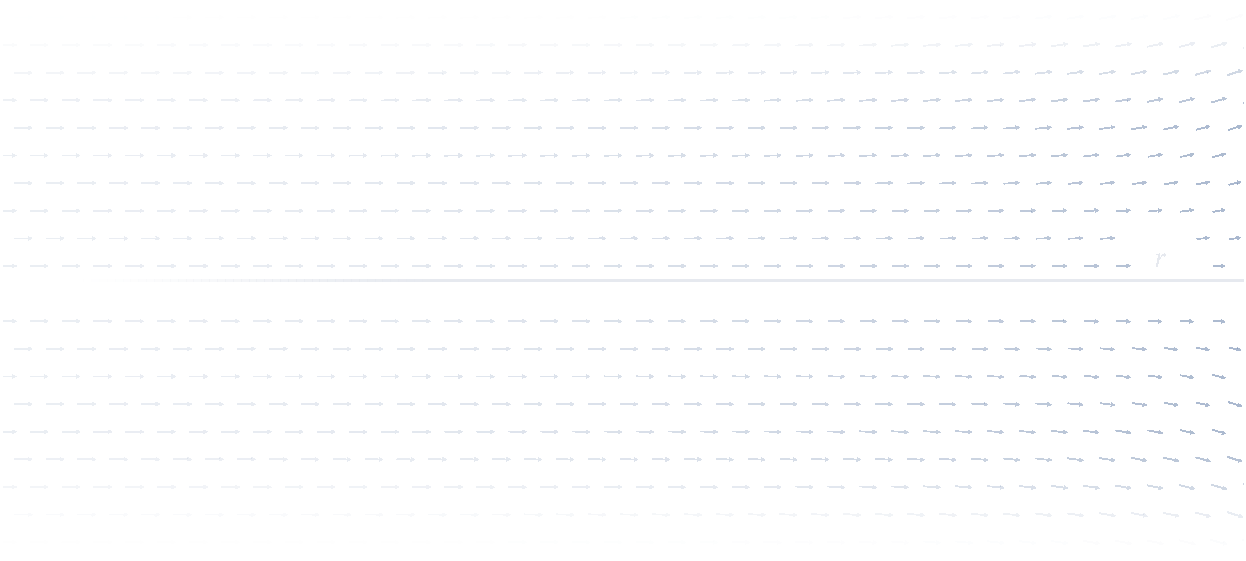
\includegraphics[width=\paperwidth]{figures/out/back_field.pdf}};
  % what the book is
  \node[anchor=north, inner sep=0pt, text=accent] at ($(current page.north)+(0,-30mm)$)
    {\sanscaps\addfontfeatures{LetterSpace=32}\small A COURSE IN FEEDBACK CONTROL};
  \node[anchor=north, inner sep=0pt, text=nighttext, align=center,
        font=\displayserif\itshape\fontsize{19}{25}\selectfont] at ($(current page.north)+(0,-40mm)$)
    {“The controller never sees the wind.\\
     It only reacts to the error it causes.”};
  \node[anchor=north, inner sep=0pt, text=nighttext] at ($(current page.north)+(0,-64mm)$)
    {\parbox{132mm}{\rmfamily\fontsize{11.2}{16}\selectfont\centering
     \emph{Anemostatos} is a course in feedback control, from PID to learning, and the companion to
     an open-source simulator in which a quadrotor has to stand still in the wind. It is built
     from the particular to the general: thirty-five lessons, one idea each, flown at three levels
     of reality, from a single vertical axis to a full quadrotor on four motors. Every figure in
     the book was flown in the simulator, and any number it attributes to the
     simulator can be reproduced by running the lesson.\par}};
  % what the reader will be able to do
  \node[anchor=north, inner sep=0pt, text=nightmuted] at ($(current page.north)+(0,-199mm)$)
    {\sanscaps\addfontfeatures{LetterSpace=24}\scriptsize WHAT YOU WILL BE ABLE TO DO};
  \node[anchor=north, inner sep=0pt, text=nighttext] at ($(current page.north)+(0,-206mm)$)
    {\parbox{132mm}{\sffamily\small\linespread{1.3}\selectfont\centering
     \setlength{\parskip}{2.2mm}
     explain every term of a PID controller physically,\\ and predict its behaviour with a few lines of algebra\par
     diagnose the classic practical problems of a loop from a plot\par
     tune a cascade of loops for a vehicle that moves in three dimensions\par
     say what the modern alternatives to PID do,\\ what each of them costs, and how to choose between them\par}};
  % the simulator
  \node[anchor=south, inner sep=0pt, text=nighttext] at ($(current page.south)+(0,35mm)$)
    {\ttfamily\fontsize{11}{13}\selectfont github.com/wojciech-stelmaszewski/anemostatos};
  % the band of the front
  \fill[accent] ($(current page.south west)+(0,13mm)$) rectangle ($(current page.south east)+(0,27mm)$);
  \node[anchor=west, inner sep=0pt, text=night] at ($(current page.south west)+(16mm,20mm)$)
    {\sanscaps\addfontfeatures{LetterSpace=20}\scriptsize THIRTY-FIVE LESSONS};
  \node[anchor=east, inner sep=0pt, text=night] at ($(current page.south east)+(-16mm,20mm)$)
    {\sanscaps\addfontfeatures{LetterSpace=20}\scriptsize THREE LEVELS OF REALITY};
\end{tikzpicture}
\null
